\paragraph{QuizziPedia::Front-End::Directives::SearchDirective}

\label{QuizziPedia::Front-End::Directives::SearchDirective}

\begin{figure}[h]
	\centering
	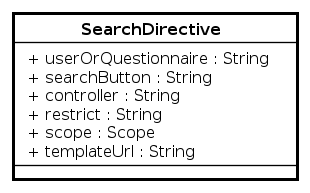
\includegraphics[scale=0.80,keepaspectratio]{UML/Classi/Front-End/QuizziPedia_Front-end_Directives_SearchDirective.png}
	\caption{QuizziPedia::Front-End::Directives::SearchDirective}
\end{figure}

\begin{itemize}
	\item \textbf{Descrizione}: \textit{directive\ped{G}} che permette di effettuare la ricerca di utenti e questionari;
	\item \textbf{Utilizzo}: permette all'utente di effettuare ricerche, è formata da:
	\begin{itemize}
		\item Barra di ricerca;
		\item Pulsante per effettuare la ricerca.
	\end{itemize}
	\item \textbf{Relazioni con altre classi}:
	\begin{itemize}
		\item \textbf{OUT \texttt{HomeView}}: \textit{view\ped{G}} contenente la barra di ricerca per gli utenti e questionari e il bottone che porterà l'utente nella modalità allenamento;
		\item \textbf{OUT \texttt{MenuBarDirective}}: rappresenta il menù, presente in ogni pagina dell'applicazione, generato in base agli oggetti passati nello \$scope isolato. Fornisce un pulsante per ogni oggetto ricevuto come parametro, ogni pulsante viene rappresentato con un'icona e con un testo. Al click di un pulsante viene invocata la funzione ad esso associata;
		\item \textbf{IN \texttt{ResultsModelView}}: classe di tipo \textit{modelview\ped{G}} la cui istanziazione è contenuta all'interno della variabile di ambiente \$scope di \textit{Angular\ped{G}}. All'interno di essa sono presenti le variabili e i metodi necessari per il \textit{Two-Way Data-Binding\ped{G}} tra la \textit{view\ped{G}} \texttt{ResultsView}, la \textit{directive\ped{G}} \texttt{SearchDirective} e il \textit{controller\ped{G}} \texttt{ResultsController};
		\item \textbf{IN \texttt{LangModel}}: rappresenta il modello delle informazioni per la giusta traduzione dell'applicazione.
	\end{itemize}
	\item \textbf{Attributi}:
	\begin{itemize}
		\item \texttt{+ userOrQuestionnaire: String} \\ Attributo che contiene l'informazione cercata;
		\item \texttt{+ searchButton: String} \\ Attributo che viene utilizzato per visualizzare la giusta traduzione della \textit{label\ped{G}} per il bottone di ricerca, in italiano o in inglese;
		\item \texttt{+ controller: String} \\ Stringa contenente il nome del \textit{controller\ped{G}} della direttiva;
		\item \texttt{+ restrict: String} \\ Stringa che permette di definire le modalità di inserimento della direttiva all'interno della pagina;
		\item \texttt{+ scope: Scope} \\ Oggetto scope interno della direttiva, contiene le funzionalità per gestire i dati presenti all'interno;
		\item \texttt{+ templateUrl: String} \\ Stringa contenente il percorso del file \textit{HTML\ped{G}} che contiene la direttive.
	\end{itemize}
\end{itemize}